\documentclass[10pt]{article}

\usepackage[utf8]{inputenc}
\usepackage[english]{babel}
\usepackage{fullpage}
\usepackage{setspace}
\usepackage{parskip}
\usepackage{titlesec}
\usepackage[section]{placeins}
\usepackage{xcolor}
\usepackage{breakcites}
\usepackage{lineno}


\PassOptionsToPackage{hyphens}{url}
\usepackage[colorlinks = true,
            linkcolor = blue,
            urlcolor  = blue,
            citecolor = blue,
            anchorcolor = blue]{hyperref}
\usepackage{etoolbox}
\makeatletter
\makeatother
\usepackage[
	backend=biber,
	style=authoryear,
	natbib=true,
	doi=false,isbn=false,url=false,eprint=false,date=year
	]{biblatex}
	
\renewcommand\nameyeardelim{, }
\addbibresource{../library.bib}

\renewenvironment{abstract}
  {{\bfseries\noindent{\abstractname}\par\nobreak}\footnotesize}
  {\bigskip}

\titlespacing{\section}{0pt}{*3}{*1}
\titlespacing{\subsection}{0pt}{*2}{*0.5}
\titlespacing{\subsubsection}{0pt}{*1.5}{0pt}

\usepackage{authblk}
\usepackage[pdftex]{graphicx}
\usepackage{tcolorbox}
\usepackage{graphicx}
\usepackage[space]{grffile}
\usepackage{latexsym}
\usepackage{textcomp}
\usepackage{longtable}
\usepackage{tabulary}
\usepackage{booktabs,array,multirow}
\usepackage{amsfonts,amsmath,amssymb}
\providecommand\citet{\cite}
\providecommand\citep{\cite}
\providecommand\citealt{\cite}
% You can conditionalize code for latexml or normal latex using this.
\newif\iflatexml\latexmlfalse
\providecommand{\tightlist}{\setlength{\itemsep}{0pt}\setlength{\parskip}{0pt}}%
\AtBeginDocument{\DeclareGraphicsExtensions{.pdf,.PDF,.eps,.EPS,.png,.PNG,.tif,.TIF,.jpg,.JPG,.jpeg,.JPEG}}
\usepackage{float}


\begin{document}

\title{\textbf{Appendix A (Social Feedback and the Adaptive Value of Information in a Dynamic Game of Divorce)}}

\author[1]{Tristan J Canterbury}%
\author[1]{Sasha RX Dall}%
\author[1]{Alex Thornton}%
\author[2]{John M McNamara}%
\affil[1]{Centre for Ecology and Conservation, University of Exeter}%
\affil[2]{School of Mathematics, University of Bristol}%
\vspace{-1em}
\date{January 21, 2024}

% Formatting title and authors
\begingroup
\let\center\flushleft
\let\endcenter\endflushleft
\maketitle
\endgroup

\selectlanguage{english}


\section{The Model}

\begin{figure}
	\centering
	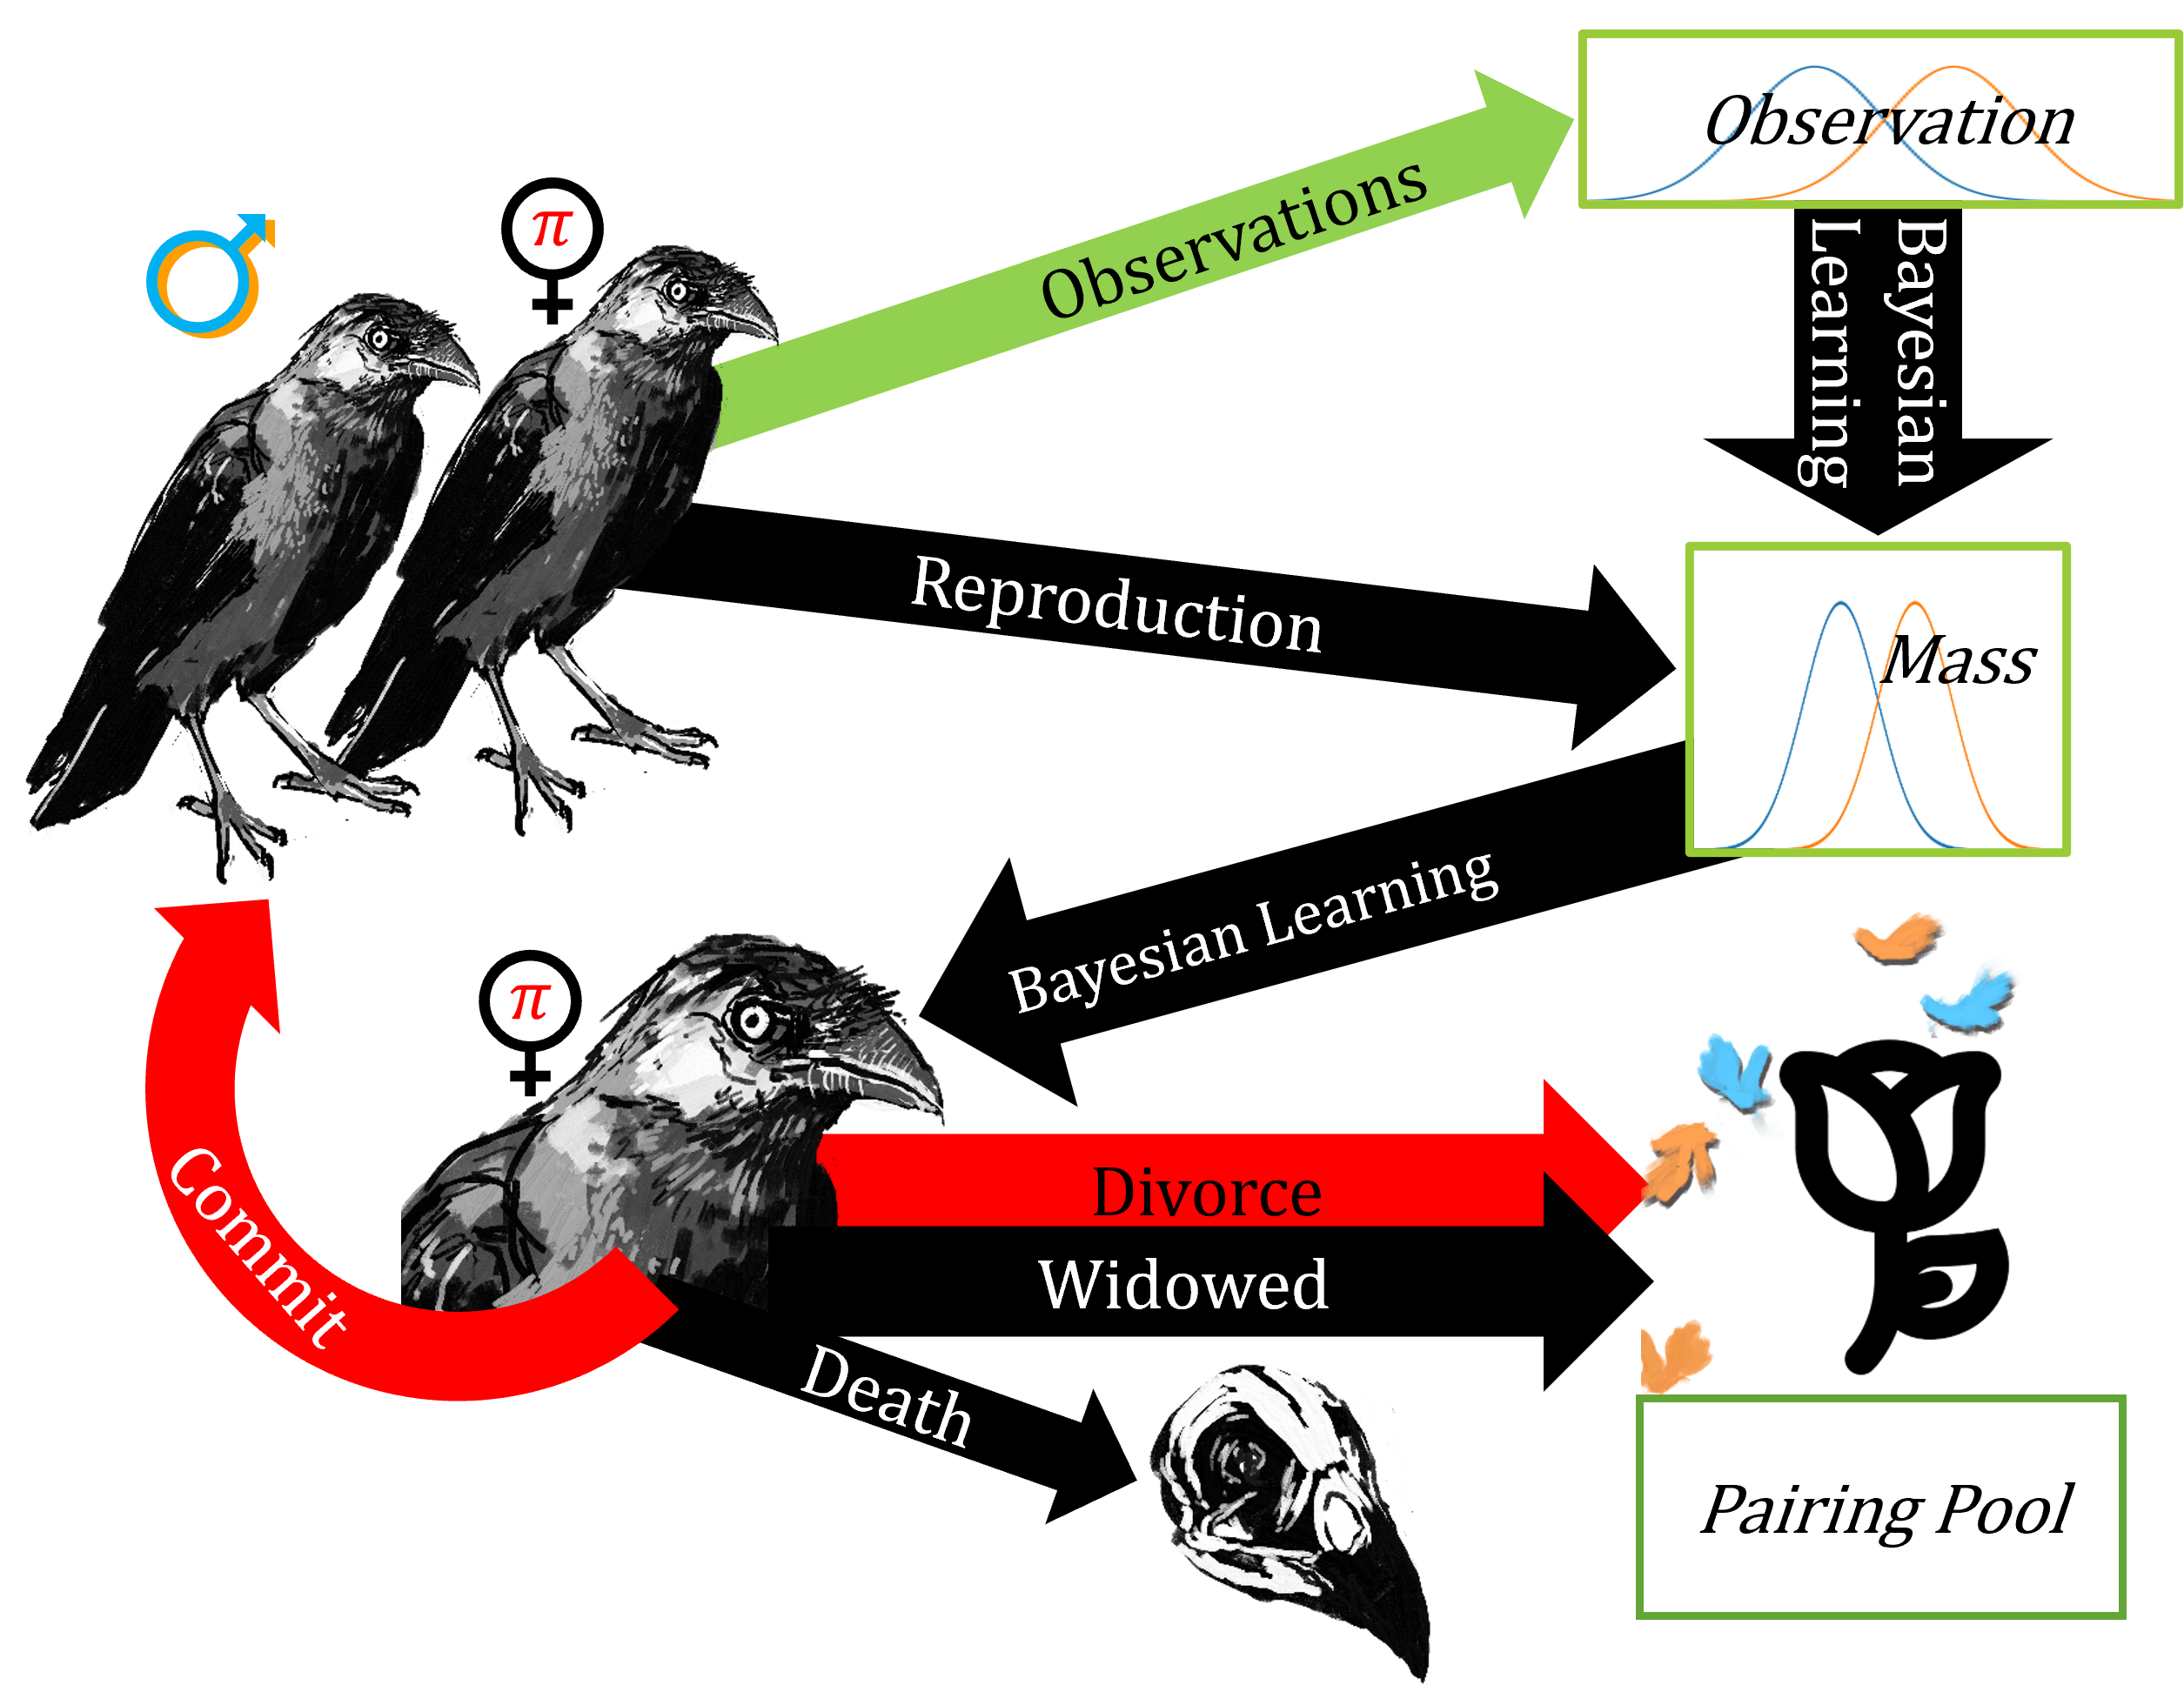
\includegraphics[width=0.8\textwidth]{../Picture1.png}
\end{figure}

I consider a population in which females follow the strategy set $(x,\psi)$.
Females have an observation strategy $\psi$ which is dependent on
their belief state $\pi$. At cost to their own contribution to offspring
mass, females can increase the proportion of their time, denoted by
$\psi(\pi)$, dedicated to observation of partner ability prior to
offspring fledgling, generating the posterior belief state $\mu$.
Females then have a divorce strategy $x$ dependent on $\mu$, with
$x(\mu)$ giving the probability of divorce. Let $\eta_{x}(t)$ be
the proportion of high ability males in the pairing pool in year $t$.
I outline a procedure for calculating 
\begin{equation}
	\tilde{\eta}(x)=\underset{t\rightarrow\infty}{\lim}\eta_{x}(t)\label{eq:}
\end{equation}


\subsection{The grid of $M$ values }

In calculating posteriors after breeding it will be convenient to
suppose that the offspring have mass
\begin{equation}
	M=a_{f}+a_{m}+\epsilon\label{eq:-1}
\end{equation}

where the random variable $\epsilon$ takes discrete values which
approximate a normal distribution. This is because all calculations
need to be on a discrete grid, and also because when we have a discrete
random variable we can work with probability mass functions rather
than probability density functions.

We assume that the observation information is garbled offspring mass
information, with the same mean but greater variance. The informativeness
of the observation is increased the longer the partner is observed,
where $\psi(\pi)=z/Z$ $z\in\{0,1,2,...,(Z-1),Z\}$ is the observation
strategy. for each $z>0$
\begin{equation}
	\sigma_{z}=Z-z+\sigma\label{eq:-9-1}
\end{equation}

so that when $z=Z$, the variation of the observation distribution
is equal to variance of offspring mass. Where there is no observation,
$z=0$, the observation distribution is
\begin{equation}
	q_{i,z}=\frac{1}{2G}\label{eq:-10-1}
\end{equation}

and when $z>0$ or the source is offspring mass ($z=Z$), the information
distribution is
\begin{equation}
	\begin{array}{ccc}
		\mathbb{P}(\epsilon=i/N)\equiv q_{i,z}=\frac{1}{K}e^{-\frac{(i/N)^{2}}{2\sigma_{z}^{2}}} & \text{for} & -G<i<G+G_{0},\end{array}\label{eq:-2}
\end{equation}
where 
\[
K=\underset{-G}{\overset{G}{\boldsymbol{\sum}}}e^{-\frac{(i/N)^{2}}{2\sigma_{z}^{2}}}
\]
Here $N$ is a suitable integer that determines the fineness of the
grid of values and $G$ determines the range. Computations might be
based on, say, $N=20$, $\sigma=1$, and $G=100$, so that the range
includes 5 standard deviations. 

\subsection{Offspring Mass Information}

For a female of given ability $F$, using resident observation strategy
$\psi$ (which takes values from between 0 and 1), It will be convenient
to assume that the two possible male abilities, $a_{L}$ and $a_{H}$,
satisfy 
\[
a_{H}-a_{L}=\frac{G_{0}}{N},
\]
where $G_{0}$ is a positive integer which satisfies $G_{0}<2G$.
Set 
\begin{equation}
	\begin{array}{ccc}
		m_{i}=F(1-\psi(j/J))+a_{L}+\frac{i}{N} & \text{for} & -G\leq i\leq G+G_{0}\end{array}.\label{eq:-4}
\end{equation}
However, we can assume that the female knows her own contribution,
$F(1-\psi(j/J))$, and so she updates her beliefs conditional on this.
\[
\begin{array}{ccc}
	P(M=m_{i}|A=a_{L})=q_{i} & \text{for} & -G\leq i\leq G\end{array},
\]
\[
\begin{array}{ccc}
	P(M=m_{i}|A=a_{H})=q_{i-G_{0}} & \text{for} & -G+G_{0}\leq i\leq G+G_{0}\end{array},
\]
where the random variable $A$ denotes the ability of the male. Note
that the probabilities of values of $m_{i}$ outside of these ranges
are zero. where the likelihood ratio is given by 
\begin{multline*}
	l_{i}=\frac{P(M=m_{i}|A=a_{H})}{P(M=m_{i}|A=a_{L})}\\
	\begin{array}{ccc}
		=\frac{q_{i-G_{0}}}{q_{i}}, & \text{for} & -G+G_{0}\leq i\leq G\end{array}
\end{multline*}


\subsection{Observation Information }

We assume that this information source is less informative than offspring
mass and so we model it as a garbled offspring mass. The informativeness
of the observation is increased the longer the partner is observed,
where $\psi(\pi)=z/Z$ is the observation strategy, where $z\in\{0,1,2,...,(Z-1),Z\}$,
giving a normal distribution of same mean as mass distribution and
a standard deviation defined as
\begin{equation}
	\sigma_{z}=Z-z+\sigma\label{eq:-9}
\end{equation}

when $z>0$, so that when $z=Z$, the variation of the observation
distribution is equal to variance of offspring mass. Where there is
no observation, $z=0$, the observation distribution is
\begin{equation}
	q_{i,z}=\frac{1}{2G}\label{eq:-10}
\end{equation}

We can then find the likelihood ratio as before
\begin{equation}
	\check{l}_{i,z}=\begin{array}{ccc}
		\frac{\check{q}_{i-G_{0},z}}{\check{q}_{i,z}}, & \text{for} & -G+G_{0}\leq i\leq G\end{array}\label{eq:-11}
\end{equation}


\subsection{Bayesian Updating}

Computations need to be based on discrete values for the posteriors.
The simplest idea would be to assume that prior and posterior values
lie on the grid
\[
0,1/J,2/J,...,(J-1)/J,1,
\]
where $J$ is an integer (say, $J=1000$). 

\subsubsection{Observation Information}

Suppose an individual has some prior belief $j/J$. Prior to breeding,
a female with observation strategy will receive some message $i$
from her observations and will update her belief, generating the posterior
belief $\pi_{i,z}(j/J)$ like so
\[
\begin{array}{ccc}
	\pi_{i,z}(j/J)=0 & \text{for} & -G\leq i<-G+G_{0},\end{array}
\]
\[
\begin{array}{ccc}
	\pi_{i,z}(j/J)=\frac{j/J\check{l}_{i,z}}{(1-j/J)+j/J\check{l}_{i,z}} & \text{for} & -G+G_{0}\leq i\leq G,\end{array}
\]
\[
\begin{array}{ccc}
	\pi_{i,z}(j/J)=1 & \text{for} & G+1\leq i\leq G+G_{0},\end{array}.
\]

Suppose that before observation and breeding the prior probability
that the male is high ability is $j/J$. Also suppose that observation
strategy $\psi$ is used. After breeding the mass of offspring is
$M=m_{i}$. Then the exact value of the posterior is $\pi{}_{i,z}(j/J)$.
However, this will typically not be on the discrete grid. Define the
integers 
\[
n^{(1)}(j,i,z)=\text{floor }\{J\pi{}_{i,z}(j/J)\},
\]
\[
n^{(2)}(j,i,z)=\text{min}\{n^{(1)}(j,i,z)+1;J\}.
\]
Also define the probabilities
\[
p^{(2)}(j,i,z)=J\pi{}_{i,z}(j/J)-n^{(1)}(j,i,z),
\]
\[
p^{(1)}(j,i,z)=1-p^{(2)}(j,i,z).
\]
Then we can approximate by assuming that the posterior is either $n^{(1)}(j,i,z)/J$
with probability $p^{(1)}(j,i,z)$ or is $n^{(2)}(j,i,z)/J$ with
probability $p^{(2)}(j,i,z)$. 
\begin{itemize}
	\item For each $j$: define $z=\psi(j/J)$ and
	\begin{itemize}
		\item For each $i$ in the range $-G\leq i\leq G$: add $\check{q}_{i,z}p^{(1)}(j,i,z)$
		to $a_{j,n^{(1)}(j,i,z),L}(z)$. 
		\item For each $i$ in the range $-G\leq i\leq G$: add $\check{q}_{i,z}p^{(2)}(j,i,z)$
		to $a_{j,n^{(2)}(j,i,z),L}(z)$
		\item For each $i$ in the range $-G+G_{0}\leq i\leq G+G_{0}$: add $\check{q}_{i-G_{0},z}p^{(1)}(j,i,z)$
		to $a_{j,n^{(1)}(j,i,z),H}(z)$ 
		\item For each $i$ in the range $-G+G_{0}\leq i\leq G+G_{0}$: add $\check{q}_{i-G_{0},z}p^{(2)}(j,i,z)$
		to $a_{j,n^{(2)}(j,i,z),H}(z)$
	\end{itemize}
\end{itemize}
Where $a_{j,u,L}(z)$ and $a_{j,u,H}(z)$ are the transition probabilities
from belief $j/J$ to belief $u/J$ given observation $z$ of the
partners that are $L$ and $H$ respectively.

\subsubsection{Mass Information}

This is then also the probability that her partner will be of high
ability at time of breeding. After breeding, she will update her belief
again from message $i$ from her offspring fledgling mass. Her posterior
belief after updating will be $\pi_{i}(\mu)$ calculated likewise
\[
\begin{array}{ccc}
	\pi{}_{i}(\mu)=0 & \text{for} & -G\leq i<-G+G_{0},\end{array}
\]
\[
\begin{array}{ccc}
	\pi{}_{i}(\mu)=\frac{\pi l_{i}}{(1-\pi)+\pi l_{i}} & \text{for} & -G+G_{0}\leq i\leq G,\end{array}
\]
\[
\begin{array}{ccc}
	\pi{}_{i}(\mu)=1 & \text{for} & G<i\leq G+G_{0},\end{array}
\]
This belief is then used as her informational state by which she makes
her divorce decision.

Suppose that before observation and breeding the prior probability
that the male is high ability is $j/J$. Also suppose that observation
strategy $\psi$ is used. After breeding the mass of offspring is
$M=m_{i}$. Then the exact value of the posterior is $\pi{}_{i}(j/J)$.
However, this will typically not be on the discrete grid. Define the
integers 
\[
n^{(1)}(i,j)=\text{floor }\{J\pi{}_{i}(j/J)\},
\]
\[
n^{(2)}(i,j)=\text{min}\{n^{(1)}(i,j)+1;J\}.
\]
Also define the probabilities
\[
p^{(2)}(i,j)=J\pi{}_{i}(j/J)-n^{(1)}(i,j),
\]
\[
p^{(1)}(i,j)=1-p^{(2)}(i,j).
\]
Then we can approximate by assuming that the posterior is either $n^{(1)}(i,j)/J$
with probability $p^{(1)}(i,j)$ or is $n^{(2)}(i,j)/J$ with probability
$p^{(2)}(i,j)$. 
\begin{itemize}
	\item For each $j$: define $z=\psi(j/J)$ and
	\begin{itemize}
		\item For each $i$ in the range $-G\leq i\leq G$: add $q_{i}p^{(1)}(i,j)$
		to $b_{u,n^{(1)}(i,j),L}$. 
		\item For each $i$ in the range $-G\leq i\leq G$: add $q_{i}p^{(2)}(i,j)$
		to $b_{u,n^{(2)}(i,j),L}$
		\item For each $i$ in the range $-G+G_{0}\leq i\leq G+G_{0}$: add $q_{i-G_{0}}p^{(1)}(i,j)$
		to $b_{u,n^{(1)}(i,j),H}$ 
		\item For each $i$ in the range $-G+G_{0}\leq i\leq G+G_{0}$: add $q_{i-G_{0}}p^{(2)}(i,j)$
		to $b_{u,n^{(2)}(i,j),H}$
	\end{itemize}
\end{itemize}
Where $b_{u,k,L}$ and $b_{u,k,H}$ are the transition probabilities
from belief $u/J$ to belief $k/J$ given the partners are $L$ and
$H$ respectively.

\subsection{Iterating forward over one year }

I assume that that the population is large and that there are equal
numbers of males and females. A proportion $1-\beta$ of offspring
that survive to enter their first breeding season are low ability
and a proportion $\beta$ are high ability. The probability of death
overwinter, $d$, is the same for males and females, and for males
does not depend on ability. Since the population is of constant size,
relative to the number of females in the breeding population, $(1-\beta)d$
L males and $\beta d$ H males enter the breeding population each
year. 

At the beginning of a breeding season we can decompose the female
population into the following proportions: 
\[
\rho_{H}(j)=\text{proportion of females with a H male and her prior he is H}=j/J,
\]
\[
\rho_{L}(j)=\text{\text{proportion of females with a L male and her prior he is H}}=j/J.
\]
Note that these are proportions of the entire female population so
that. 
\[
\underset{j}{\boldsymbol{\sum}}\rho_{L}(j)=1-\beta,
\]
\[
\underset{j}{\boldsymbol{\sum}}\rho_{H}(j)=\beta.
\]
Let $\tilde{\rho}_{H}$ and $\tilde{\rho}_{L}$ denote the corresponding
posterior arrays after breeding. We may find these as follows: 

Suppose that $k/J$ is the posterior beliefs of individuals after
both observation and offspring mass information has been received.
For each $k$: define $z=\psi(j/J)$ and

\begin{equation}
	P(k|j,z,L)=\underset{u}{\sum}a_{j,u,L}(z)b_{u,k,L}\label{eq:-5}
\end{equation}

\begin{equation}
	P(k|j,z,H)=\underset{u}{\sum}a_{j,u,H}(z)b_{u,k,H}\label{eq:-5-1}
\end{equation}

\begin{equation}
	\tilde{\rho}_{L}(k)=\underset{j}{\sum}\rho_{L}(j)P(k|j,z,L)\label{eq:-6}
\end{equation}

\begin{equation}
	\tilde{\rho}_{H}(k)=\underset{j}{\sum}\rho_{H}(j)P(k|j,z,H)\label{eq:-7}
\end{equation}

These are also proportions and so should satisfy $\forall j$
\[
\underset{j}{\boldsymbol{\sum}}\tilde{\rho}_{L}(j)=1-\beta,
\]
\[
\underset{j}{\boldsymbol{\sum}}\tilde{\rho}_{H}(j)=\beta.
\]
Assume that the resident divorce strategy $x$, the relative number
(relative to the total number of females in a breeding population)
of L and H males that are divorced after breeding are 
\[
D_{L}=\underset{j}{\boldsymbol{\sum}}\tilde{\rho}_{L}(j)x(j/J),
\]
\[
D_{H}=\underset{j}{\boldsymbol{\sum}}\tilde{\rho}_{H}(j)x(j/J),
\]
and the relative number (relative to the total number of females in
a breeding population) of L and H males that are not divorced after
breeding are 
\[
M_{L}=\underset{j}{\boldsymbol{\sum}}\tilde{\rho}_{L}(j)(1-x(j/J)),
\]
\[
M_{H}=\underset{j}{\boldsymbol{\sum}}\tilde{\rho}_{H}(j)(1-x(j/J)),
\]
The pairing pool next year comprise: 
\begin{itemize}
	\item These individuals, if they survive 
	\item Individual that are not divorced, but lose their female partner through
	death and survive themselves 
	\item New male offspring entering the pool for the first time. 
\end{itemize}
Thus the relatives numbers of L and H males (relative to the total
number of females in a breeding population) in the pool are
\[
\alpha_{L}=(1-d)D_{L}+d(1-d)M_{L}+(1-\beta)d,
\]
\[
\alpha_{H}=(1-d)D_{H}+d(1-d)M_{H}+\beta d.
\]
Thus, in the pairing pool a proportion $\eta'=\alpha_{H}/(\alpha_{H}+\alpha_{L})$
of those males present are H. 

In the new breeding season the prior probability that a newly acquired
male is H is $\eta'$. As above, we can let $j_{1}$ be the integer
part of $J\eta'$, let $j_{2}=\text{min}\{j_{1}+1,J\}$, set $s_{2}=J\eta'-j_{1}$,
and set $s_{1}=1-s_{2}$. Let
\[
\begin{array}{ccc}
	\bar{\rho}(j)=s_{1} & if & j=j_{1}\end{array}
\]
\[
\begin{array}{ccc}
	\bar{\rho}(j)=s_{2} & if & j=j_{2}\end{array}
\]
\[
\begin{array}{ccc}
	\text{else} & \bar{\rho}(j)=0\end{array}
\]
Then relative numbers of females with L and H males and with the
appropriate posteriors are 

\begin{equation}
	\rho'_{L}(j)=\tilde{\rho}_{L}(j)[1-x(j/J)](1-d)^{2}+\alpha_{L}\bar{\rho}(j)\label{eq:-2-1}
\end{equation}

\begin{equation}
	\rho'_{H}(j)=\tilde{\rho}_{H}(j)[1-x(j/J)](1-d)^{2}+\alpha_{H}\bar{\rho}(j)\label{eq:-3}
\end{equation}
As a check we should then have 
\[
\underset{j}{\boldsymbol{\sum}}\rho'_{L}(j)=1-\beta,
\]
\[
\underset{j}{\boldsymbol{\sum}}\rho'_{H}(j)=\beta.
\]


\subsection{Iterating to convergence }

If we start with some initial functions $\rho_{L}$ and $\rho_{H}$
we can use the above to calculate the corresponding quantities next
year, and so on for all future years. I expect the successive iterate
to convergent to a limit. Numerically if we set 
\[
\text{diff}=\underset{j}{\boldsymbol{\sum}}(|\rho_{L}(j)-\rho'_{L}(j))|+|\rho_{H}(j)+\rho'_{H}(j)|)
\]
as a measure of the difference in successive year, then we continue
until diff is less than some tolerance (e.g. $\text{tol}=10^{-6}$).
I also expect the limit to be independent of the starting functions
(should check this when the program runs). As $\rho$ converges, so
should $\eta$.

\subsection{Best Response}

Having found $\tilde{\eta}(x,\psi)$, we can use this to determine
the fitness outcome of entering the pairing pool and so the find the
best response in terms of observation and divorce strategy, $\hat{b}(x,\psi)(j/J)$. 

\subsection{Offspring Mass}

We first must know the probability of each offspring mass for a given
prior belief that partner ability is high, $j/J$. For now we assume
that all variation in female ability is contributed by their observation
strategies. So offspring mass at fledgling for a pair, with female
observation strategy $\psi(j/J)=z/Z$ and prior belief $j/J$, will
be 
\[
m_{i}(z)=F(1-z/Z)+a+\frac{i}{N}\text{ }\forall i.
\]
Where $F$ is female ability and $a\in\{L,H\}$ is male ability. As
some individuals are able to become misinformed (e.g. $\rho_{L}(J)>0$)
we must calculate the true probability that an individual is with
a partner of ability $H$ whenof belief $j/J$, which can be defined
as $\forall j$
\[
T(j)=P(H|j)=\frac{\rho_{H}(j)}{\rho_{L}(j)+\rho_{H}(j)}
\]

Interestingly the degree of misinformation may vary with the quality
of information. To calculate $\mathbb{P}(i|j)$ (the probability of
mass $m_{i}(z)$ given prior belief state $j$) first set $\forall j\forall i$
$\mathbb{P}(i|j)=0$, then $\forall j$
\begin{itemize}
	\item for $i$ in the range $-G\leq i\leq G$: add $(1-P(H|j))q_{i}$ to
	$\mathbb{P}(i|j)$.
	\item for $i$ in the range $-G+G_{0}\leq i\leq G+G_{0}$: add $P(H|j)q_{i-G_{0}}$
	to $\mathbb{P}(i|j)$.
\end{itemize}
We can use this to find the mean mass of offspring at fledgling individuals
of belief state $j$
\begin{equation}
	R(j,z)=\underset{i}{\sum}m_{i}(z)P(i|j),\label{eq:-5-2}
\end{equation}
giving us this breeding season's contribution to the female's lifetime
reproductive success $V_{n}$. 

\subsection{Bayesian Updating}

We next need to update the individual's beliefs. $\mathbb{P}(k|j,z)$
is the transition probability from belief $j/J$ to belief $k/J$,
given observation strategy $\psi(j/J)=z$ and offspring mass information.
For Bayesian updating from observation and offspring mass $\forall j\forall z$

\begin{equation}
	P(k|j,z)=(j/J)P(k|j,z,H)+(1-j/J)P(k|j,z,L)\label{eq:-6-1}
\end{equation}


\subsection{Expected Divorce Outcomes}

The next event in the annual cycle is the census event in which individuals
are divorced or die, causing the focal individual to enter the pairing
pool. If an individual were to enter the pairing pool we know that
their posterior belief distribution on the discrete grid shall be
$k_{1}=floor\{J\tilde{\eta}(x)\},$ and $k_{2}=min\{k_{1}+1,J\}$
with probabilities $u_{2}=J\tilde{\eta}(x)-k_{1}$, and $u_{1}=1-u_{2}$
for $k_{2}$ and $k_{1}$ respectively. These will determine the expected
fitness outcome $H_{P}$ for entering the pairing pool, assuming they
survive to next breeding season
\begin{equation}
	H_{P}=u_{1}V_{n-1}(k_{1})+u_{2}V_{n-1}(k_{2}).\label{eq:-4-1-1}
\end{equation}

The expected fitness outcomes for choosing to divorce $H_{D}$ and
choosing to remain coupled $H_{C}$ are simply
\[
H_{D}=(1-\varrho)H_{P},
\]
\begin{equation}
	H_{C}(k)=(1-d)[dH_{P}+(1-d)V_{n-1}(k)].\label{eq:-3-1-1}
\end{equation}

where $\varrho$ is the divorce specific death probability (typically
$\varrho\equiv d$). 

\subsection{Optimal Decision Making}

The fitness $V_{n}(j)$ given optimal decision making on iteration
$n$ and given prior belief $j/J$ is
\begin{equation}
	V_{n}(j)=\underset{z}{max}\{R(j,z)+\underset{k}{\sum}\mathbb{P}(k|j,z)\underset{}{max}\{(H_{D},H_{C}(k))\}\}.\label{eq:-4-1}
\end{equation}

To find the best response to the resident strategy then we iterate
to convergence 
\begin{equation}
	V^{*}(j)=\underset{n\rightarrow\infty}{\lim}V_{n}(j).\label{eq:-3-1}
\end{equation}
giving 
\begin{equation}
	H_{D}^{*}=(1-d)[u_{1}k_{1}V^{*}(k_{1})+u_{2}k_{2}V^{*}(k_{2})],\label{eq:-4-1}
\end{equation}
\begin{equation}
	H_{C}^{*}(k)=(1-d)[\frac{dH_{D}^{*}}{1-d}+(1-d)V^{*}(k)].\label{eq:-3-1}
\end{equation}

As the expected fitness benefit for divorcing and not divorcing. The
best response $\hat{b}(x)(j/J)$ as $n\rightarrow\infty$, defined
on the grid by 
\begin{equation}
	\hat{b}(x)(j/J)=1\;\text{ if }\;H_{D}^{*}>H_{C}^{*}(j)\label{eq:-2-2}
\end{equation}
\begin{equation}
	\hat{b}(x)(j/J)=0\;\text{ if }\;H_{D}^{*}<H_{C}^{*}(j),\label{eq:-1-1}
\end{equation}

and similarly for the best response observation strategy 
\[
\hat{b}(\psi)(j/J)=\frac{\underset{z}{argmax}\{R(j,z)+\underset{k}{\sum}\mathbb{P}(k|j,z)\underset{}{max}\{(H_{D},H_{C}(k))\}\}}{Z}.
\]


\subsection{Finding the ESS}

Next we can iterate over invasions. An invasion is simply the best
response becoming the new resident strategy $(x(j/J)=\hat{b}(x)(j/J),\psi(j/J)=\hat{b}(\psi)(j/J))$
for which a new best response must be calculated. To find the evolutionary
stable strategy we iterate over invasions until
\begin{equation}
	\hat{b}(x,\psi)(j/J)=(x,\psi)(j/J)\text{ }\forall j.\label{eq:-8}
\end{equation}


\subsection{Mapping The Information Niche Landscape}

Once we had a method for finding the optimal Information gathering
strategy for a given location in the parameter space we used a simple
hill climbing algorithm at different locations to find local information
value optima, so as to better understand the multivariable effects. 

To do this we take random samples of the the parameter space and for
each deploy a hill climbing algorithm, using total canonical cost
of no observation as the value we are maximising. 

We found 2 distinct optima for information use, one where Information
quality and certainty are low, and one where information quality and
and certainty are high.

\selectlanguage{english}
\FloatBarrier

\printbibliography



We assume that the female knows her own contribution to offspring mass $(1-C_c)a_f$ if she used $I_\psi$, or $a_f$ otherwise. So by subtracting her contribution from the mass she needs only to detect the signal of male quality $a_m$ through the noise given by $\epsilon$. For a pseudo-normal distribution such as $\epsilon$, the probability of event $y$ is
\begin{equation}
	\begin{array}{ccc}
		P(y|\sigma,N,G) = \frac{1}{K}e^{-\frac{(y/N)^{2}}{2\sigma^{2}}} & \text{for} & -G<y<G,\end{array}\label{eq:-2}
\end{equation}
where $N$ is a suitable integer that determines the fineness of the
grid of values, $G$ determines the range, $\sigma$ is the standard deviation, and $K$ is
\[
K=\underset{-G}{\overset{G}{\boldsymbol{\sum}}}e^{-\frac{(y/N)^{2}}{2\sigma^{2}}}
\]
So the probability of observation $y$ if the male is low quality is 
\[
\begin{array}{ccc}
	P(y|L,I_\psi)= P(y|\sigma+z,N,G) & \text{for} & -G\leq y\leq G\end{array},
\]
because the observation structure is just the mass structure if the standard deviation were $\sigma+z$. If the male is high quality it is
\[
\begin{array}{ccc}
	P(y|H,I_\psi)= P(y-\delta|\sigma+z,N,G) & \text{for} & -G+\delta\leq y\leq G+\delta\end{array},
\]
because we need to simply shift the range by the difference between high and low quality males $\delta$.
A female accessing information structure $I$ will receive some message $y$ from that structure. The likelihood ratio for $I_\psi$ is 
\begin{equation}
	l_{\psi}(y)=\frac{P(y|H,I_\psi)}{P(y|L,I_\psi)},
\end{equation}
and the likelihood ratio of mass $m$ for $I_\psi$ is 
\[  
l_{M}(i)=\frac{P(i|H,I_M)}{P(i|L,I_M)}.
\]
These likelihood ratios and the female's prior knowledge state $\pi$ can then be used to generate posterior knowledge states using Bayesian learning
\[
\begin{array}{ccc}
	\pi'=0 & \text{if} & i<-G+\delta,\end{array}
\]
\[
\begin{array}{ccc}
	\pi'=\frac{\pi l}{(1-\pi)+\pi l} & \text{if} & -G+\delta\leq i\leq G,\end{array}
\]
\[
\begin{array}{ccc}
	\pi'=1 & \text{if} & i>G.\end{array}
\]
\subsection{Emergence of a stable social structure}
Ihe proportion of high quality males in the pairing pool $ \eta $ is influenced by the bottom-up effects of individual decision making. We iterate forwards over multiple breeding seasons until we find a stable value for $ \eta $, assuming that (almost) all females use the same resident strategy. In the Appendix I outline the procedure for calculating the stable proportion of high quality males in the pairing pool. I assume that the population is large and that there are equal numbers of males and females. At time 0, $ \eta_{x,\psi}(t=0) $ we will choose to be $ \beta $, the proportion of high quality unpaired males that enter their first breeding season. The starting value however shouldn't significantly effect the stable value $ \tilde{\eta}_{x,\psi}$. To calculate $\eta_{x,\psi}(t+1) $ we need to account for how mortality rate $ \mu $, quality distribution $ \beta $, and individual decision making effect this distribution over time. The probability of death overwinter, $\mu$, is the same for males and females, and for males does not depend on quality. Since the population is of constant size, relative to the number of females in the breeding population, $(1-\beta)\mu$ L males and $\beta \mu$ H males enter the breeding population each year. The male pairing pool distribution next year is determined by: 
\begin{itemize}
	\item The proportion of surviving divorced males of H and L quality . 
	\item The proportion of surviving Males that are not divorced, but lose their female partner through
	death.
	\item The proportion of new male offspring entering the pool for the first time, given the proportion of males that die each year. 
\end{itemize}
Thus the relatives proportions of L and H males in the pool are
\[
\alpha_{L}=(1-\mu)D_{L}+\mu(1-\mu)M_{L}+(1-\beta)\mu,
\]
\[
\alpha_{H}=(1-\mu)D_{H}+\mu(1-\mu)M_{H}+\beta\mu.
\]
Where $D_L$, $D_H$ are the proportions of males of low and high quality respectively who are divorced, and likewise $M_L$ and $M_H$ are those that are not divorced. Therefore 
\[ 
\eta_{t+1}=\alpha_{H}/(\alpha_{H}+\alpha_{L}) 
\] 
of those males present are high quality. In the next breeding season the prior probability that a newly acquire male is H is $\eta_{x,\psi}(t+1)$. Then the relative numbers of females with L and H males and with posteriour knowledge state $\pi$ at the beginning of the next annual cycle will be 
\begin{equation}
	\rho_{L}(\pi)=\tilde{\rho}_{L}(\pi)(1-x(\pi))(1-\mu)^{2}+\alpha_{L}\bar{\rho}(\pi)\label{eq:14}
\end{equation}
\begin{equation}
	\rho_{H}(\pi)=\tilde{\rho}_{H}(\pi)(1-x(\pi))(1-\mu)^{2}+\alpha_{H}\bar{\rho}(\pi)\label{eq:15}
\end{equation}
Where $\tilde{\rho}_{L}(\pi)$ and $\tilde{\rho}_{H}(\pi)$ are the proportions of females with knowledge state $\pi$ and paired with a male of quality low and high respectively, after the use of $I_\psi$ and $I_M$ for bayesian updating. 

\section{Results}
\subsection{Optimal Divorce Strategy}
The expected fitness outcome in a given year for a female with knowledge state $\pi$, having used observation strategy $\psi$, is
\begin{equation}
	R(\pi,\psi)=\underset{i}{\sum}m_{i,psi}(\pi P(i|H,I_\psi)+(1-\pi)P(i|L,I_\psi)),\label{eq:16}
\end{equation}
Where $m_{i,psi}$ is the offspring mass at fledging, given message $i$ from $I_M$,observation strategy $\psi$, and it's related opportunity cost on mass $C_O$. Higher values of $\pi$ generates a greater expected offspring mass. Using the calculations outlined in the appendix we found that for a given resident strategy and life history, the decision-relevant state of the pairing pool $\eta$ approaches a unique value. We use this to determine the fitness outcome of entering the pairing pool and as there is no cost to divorce per se, only a cost in bad decision making with respect to the knowledge state $\pi$, we find that the ESS divorce strategy is rather straightforward. Given that knowledge state $\pi$ determines the probability that the male is high quality, $\eta$ is the probability that their partner post-divorce will be high quality, and expected fitness outcomes increase with Male quality in a given year, the female should divorce iff 
\[
\pi<\tilde{\eta},
\]
To put it simply, the female chooses the action that maximises $\pi$, as this maximises $R(\pi,\psi)$. Hence we see that the divorce threshold and the stable pairing pool state $\tilde{\eta}$, are one and the same. Thus any factor that effects the stable state of the pairing pool also has an effect on the behaviour of females.


\subsection{Optimal Observation Strategy}

The optimal observation strategy is not so straightforward to solve for. The use of an observation does not change the expected value of the female's posterior knowledge state, instead it changes the knowledge state for the better for proportion $\pi$ of the females and for the worse for the rest, but for the latter they can use divorce to remedy this. Expected amount of change depends on the amount of uncertainty in her prior knowledge and the informativeness of the observation. To find the Observation ESS we first find the best response to a resident strategy with pairing pool distribution $\eta$, assuming optimal divorce decision making 
\begin{equation}
	\hat{b}(\psi)(\pi)=\underset{\psi}{argmax}\{R(\pi,\psi)+\underset{k}{\sum}(1-C_{\mu}\psi)\mathbb{P}(\pi'=k|\pi,\psi)\underset{}{max}\{(H_{D}(\eta),H_{C}(\pi'))\}\}, \label{eq:26-1}	
\end{equation}
where $\mathbb{P}(\pi'|\pi,\psi)$ is the state transition probability from the prior knowledge state $\pi$ to the posterior knowledge state $\pi'$ given observation strategy $\psi$, $H_{D}(\eta)$ is the fitness outcome of divorce given $\eta$ calculated for a given resident strategy (outlined in Appendix), and $H_{C}(\pi')$ is the fitness outcome of committing to the male given posterior knowledge state $\pi'$. $R(\pi,\psi)$ includes the effect of the opportunity cost of the observation, $\mathbb{P}(\pi'|\pi,\psi)$ gives the effect of informativeness, and $C_\mu \underset{}{max}\{(H_{D}(\eta),H_{C}(\pi'))\}$ gives the usability of the information received given the risk of death when making the observation and the actions available.
To find the evolutionary stable strategy we iterate over invasions of best response strategies until
\begin{equation}
	\hat{b}(x,\psi)=(x,\psi).\label{eq:26}
\end{equation}
What we find in the baseline case (see Figure \ref{fig:2}) is that it is optimal to make observations when the female has high uncertainty in her prior knowledge state, and when her knowledge state is near to the divorce threshold set by $\eta$, because this is when the probability of a decision-relevant change in knowledge state is most likely. We also find that as females grow older the probability of observing and of divorce goes down, as the probability that they know that they are paired with a high quality male goes up, plateauing due to the turnover rate of the population limiting the proportion of females that can reach certainty.

\end{document}

